\chapter{فرمنت‌ها، نرم‌افزار \eng{Praat} و فضای واکه‌ای}

هدف این جلسه آن است که از روی سیگنال صوتی، ویژگی‌های \term{آکوستیکی}{Acoustic} مانند \eng{F1} و \eng{F2} را اندازه بگیریم و آن‌ها را به ویژگی‌های \term{تولیدی}{Articulatory} مانند ارتفاع و جلو یا عقب‌بودن زبان نگاشت کنیم. ابزار عملی این کار نرم‌افزار \eng{Praat} و نتیجهٔ کار، \term{فضای واکه‌ای}{Vowel Space} است که در گفتاردرمانی، تشخیص صدای جعلی و پایش بیماری‌های عصبی به کار می‌رود.

\section{مرور کوتاه: از فرکانس پایه تا فرمنت}
جزئیات فوریه، هارمونیک‌ها و مدل منبع–فیلتر در فصل ۳ آمده است. نکته‌های مرور شده در ابتدای جلسه:

\begin{itemize}
  \item \textbf{فرکانس پایه:} اگر موجی در هر $T$ ثانیه یک دورهٔ کامل بزند، $f_0=1/T$ است. برای \eng{Pitch} تکرار قله‌های اصلی، یعنی کندترین الگوی تناوبی، را در نظر می‌گیریم. $f_0$ به \emph{منبع} (چین‌های صوتی) و فرمنت‌ها به \emph{فیلتر} (مجرای صوتی) مربوط‌اند.
  \item \textbf{\eng{Magnitude} در برابر دامنه:} ضریب فوریه عدد مختلط $X=a+jb$ است؛ اندازهٔ آن $|X|=\sqrt{a^2+b^2}$ سهم آن فرکانس در سیگنال است و زاویهٔ آن فاز. دامنهٔ زمانی سیگنال و \eng{Magnitude} طیفی یکی نیستند. در اسپکتروگرام رنگ گرم‌تر یعنی مقدار طیفی بیشتر.
  \item \textbf{تعامد:} موج‌های مبنا باید متعامد باشند تا هر کدام مؤلفه‌ای مستقل را بسنجند: ضرب داخلی دو موج صفر باشد ($\int_0^T x_1(t)x_2(t)\,dt=0$). موج‌هایی با تعداد صحیح دوره در بازهٔ $T$ (فرکانس‌های $1/T,2/T,\dots$) چنین مجموعه‌ای می‌سازند.
  \item \textbf{هارمونیک‌ها:} فرکانس‌ها $f_n=nf_0$ هستند ولی ضریب برخی می‌تواند صفر باشد؛ مثلاً موج مربعی با چرخهٔ کاری ۵۰ درصد فقط هارمونیک‌های فرد دارد.
\end{itemize}

\begin{exambox}{پرسش و پاسخ: آیا تعداد هارمونیک‌ها بی‌نهایت است؟}
از نظر ریاضی بله، اما در عمل نرخ نمونه‌برداری (نایکویست) و هدف تحلیل آن را محدود می‌کند و فقط بخش مفید طیف بررسی می‌شود.
\end{exambox}

\subsection{هارمونیک در برابر فرمنت}
هارمونیک‌ها ویژگی \emph{سیگنال تناوبی} (منبع) هستند، در حالی که \term{فرمنت‌ها}{Formants} نواحی تشدید \emph{مجرای صوتی} (فیلتر) را توصیف می‌کنند و به صورت برآمدگی‌های پوش طیفی دیده می‌شوند. با نگاه به هارمونیک‌ها نمی‌توان فهمید زبان کجاست؛ برای این کار باید فرمنت‌ها را استخراج کرد. یکی از روش‌های رایج تخمین فرمنت \term{کدگذاری پیش‌بینی خطی}{Linear Predictive Coding (LPC)} است.

\begin{table}[htbp]
\centering
\caption{مقایسهٔ اسپکتروگرام پهن‌باند و باریک‌باند}
\begin{tabular}{p{3.2cm}p{5.2cm}p{5.2cm}}
\toprule
ویژگی & \eng{Wideband} & \eng{Narrowband} \\
\midrule
طول پنجره & کوتاه‌تر (حدود ۵ میلی‌ثانیه) & بلندتر \\
تفکیک زمانی / فرکانسی & زمانی بیشتر، فرکانسی کمتر & زمانی کمتر، فرکانسی بیشتر \\
ظاهر طیف & نواحی پهن انرژی؛ فرمنت‌ها دیده می‌شوند & خطوط هارمونیکی جداگانه \\
کاربرد & دنبال‌کردن فرمنت‌ها و حرکت اندام‌ها & بررسی هارمونیک‌ها و $f_0$ \\
\bottomrule
\end{tabular}
\end{table}

چون زبان و سایر اندام‌ها سریع جابه‌جا می‌شوند، برای دیدن فرمنت‌ها از نمای پهن‌باند استفاده می‌کنیم.

\section{نگاشت ویژگی‌های آکوستیکی به ویژگی‌های تولیدی}
در پردازش گفتار معمولاً موقعیت واقعی زبان را مستقیم اندازه نمی‌گیریم؛ در عوض ویژگی‌های آکوستیکی را از صوت استخراج و برای توصیف فضای واکه‌ای به کار می‌بریم. دو فرمنت اول بیشترین نقش را دارند.

\begin{definitionbox}{نگاشت \eng{F1} و \eng{F2} به ویژگی‌های تولیدی}
\begin{itemize}
  \item \term{فرمنت اول}{F1}: رابطهٔ \emph{معکوس} با ارتفاع زبان. زبان بالاتر (واکهٔ بسته) $\Leftarrow$ \eng{F1} کمتر؛ زبان پایین‌تر (واکهٔ باز) $\Leftarrow$ \eng{F1} بیشتر.
  \item \term{فرمنت دوم}{F2}: مرتبط با جلو یا عقب بودن زبان. زبان جلوتر $\Leftarrow$ \eng{F2} بیشتر؛ زبان عقب‌تر $\Leftarrow$ \eng{F2} کمتر.
  \item \term{گرد شدن لب}{Lip Rounding}: \eng{F2} را کاهش می‌دهد.
\end{itemize}
\end{definitionbox}

\begin{correctionbox}{این رابطه‌ها تقریبی‌اند}
فرمنت‌ها تشدیدهای کل مجرای صوتی‌اند، نه یک «حفرهٔ» مشخص؛ \eng{F1} علاوه بر ارتفاع زبان به باز بودن فک و تنگی حلق نیز حساس است. به همین دلیل واکهٔ عقبی گرد مانند \eng{/u/} هم \eng{F1} هم \eng{F2} پایین دارد. پاسخ استاد به پرسش «آیا قانون ثابت است؟»: این یک قاعدهٔ کلی آواشناختی است، نه رابطه‌ای بدون استثنا؛ برای یک گروه جدید رابطه را از پیش فرض نمی‌کنیم، مقادیر واقعی را اندازه می‌گیریم و تفاوت‌ها را تفسیر می‌کنیم.
\end{correctionbox}

\begin{addedbox}{مثال عددی: لولهٔ یکنواخت و اثر طول مجرا}
مجرای خنثی را می‌توان لولهٔ یک‌سر بسته (چین‌های صوتی) و یک‌سر باز (لب‌ها) گرفت: $F_n=\dfrac{(2n-1)\,c}{4L}$ با $c\approx 35000$ سانتی‌متر بر ثانیه. برای $L=17.5$ سانتی‌متر (مرد بزرگسال): $F_1=500$، $F_2=1500$ و $F_3=2500$ هرتز. برای $L=11$ سانتی‌متر (کودک): $F_1\approx 795$ و $F_2\approx 2386$ هرتز. پس مجرای کوتاه‌تر یعنی فرمنت بالاتر، و فضای واکه‌ای باید برای هر گروه جداگانه ساخته شود.
\end{addedbox}

\section{کار عملی با \eng{Praat}}
\eng{Praat} نرم‌افزار رایگان تحلیل و برچسب‌گذاری گفتار است (\eng{Boersma} و \eng{Weenink}، آمستردام). استاد آن را برای پل زدن میان ویژگی‌های آکوستیکی و تولیدی معرفی کرد؛ تمرکز بر دو کار بود: استخراج فرمنت‌ها و برچسب‌گذاری (\eng{Annotation}).

\subsection{تحلیل صوت و اندازه‌گیری فرمنت}
استاد چند واکه («ای»، «آ»، «او») را ضبط کرد. در محیط تحلیل، شکل موج در بالا، \term{طیف‌نگاره}{Spectrogram} در پس‌زمینه، منحنی آبی \eng{Pitch} و نقطه‌های قرمز \eng{Formants} دیده می‌شود. با کلیک روی هر لحظه، فرمنت‌ها همان لحظه نمایش داده می‌شوند (در کلاس: \eng{F1} حدود ۳۴۰، \eng{F2} حدود ۲۰۰۰ و \eng{F3} حدود ۳۰۰۰ هرتز، الگوی شبیه \eng{/i/}؛ واحد هرتز است). این‌ها اندازه‌گیری یک لحظه‌اند، نه مقدار ثابت واکه.

لازم نیست فقط در یک نقطه بخوانیم: بازهٔ زمانی یک واکه (مثلاً «آ») را انتخاب، میانگین \eng{F1} و \eng{F2} را از \eng{Praat} می‌گیریم و برای تحلیل ذخیره می‌کنیم. در پژوهش‌ها معمولاً فرمنت در میانهٔ واکه (حدود ۵۰ درصد مدت) یا میانگین ۲۰ تا ۸۰ درصد خوانده می‌شود تا اثر همخوان‌های مجاور کم شود.

\begin{correctionbox}{سقف فرمنت (\eng{Maximum formant}) را بر حسب گوینده تنظیم کنید}
\eng{Praat} فرمنت‌ها را با روش \eng{Burg} (نوعی \eng{LPC}) تخمین می‌زند. راهنمای معمول با ۵ فرمنت: حدود ۵۰۰۰ هرتز برای مردان، ۵۵۰۰ (پیش‌فرض) برای زنان و مقادیر بالاتر برای کودکان. سقف نامناسب فرمنتی را حذف یا اضافه می‌کند. خروجی را همیشه با طیف‌نگاره بازبینی کنید؛ وقتی $f_0$ بالا است (زنان و کودکان) ممکن است هارمونیک به جای فرمنت انتخاب شود. برای \eng{Pitch} نیز بازهٔ جست‌وجو را متناسب با گوینده بگذارید (مردان حدود ۷۵ تا ۳۰۰ و زنان ۱۰۰ تا ۵۰۰ هرتز) وگرنه $f_0$ نصف یا دو برابر می‌شود.
\end{correctionbox}

\subsection{برچسب‌گذاری گفتار با \eng{TextGrid}}
مهم‌ترین کاربرد \eng{Praat} در این جلسه \eng{Annotation} بود: مشخص‌کردن مرزهای زمانی و برچسب‌زدن بخش‌های صوت. ساختار آن \eng{TextGrid} است و از چند لایه (\eng{Tier}) ساخته می‌شود. استاد سه سطح را مثال زد:

\begin{center}
\begin{tabular}{lccc}
\toprule
لایه & \multicolumn{3}{c}{برچسب‌ها} \\
\midrule
\eng{Word Tier} (سطح واژه) & \multicolumn{3}{c}{ای آ او} \\
\eng{Syllable Tier} (سطح هجا) & ای & آ & او \\
\eng{Phoneme Tier} (سطح واج) & \eng{/i/} & \eng{/ɑ/} & \eng{/u/} \\
\bottomrule
\end{tabular}
\end{center}

با تعیین بازهٔ هر واکه یا همخوان، علاوه بر برچسب زبانی، اطلاعات آکوستیکی همان بازه هم استخراج می‌شود. نتیجه مجموعه‌داده‌ای است که برای هر بازه می‌گوید چه واجی تولید شده، \eng{F1} و \eng{F2} آن چقدر بوده و گوینده به کدام گروه آماری تعلق دارد.

\boardfigure{0.8}{ch04-praat-textgrid.png}{نمونهٔ یک \eng{TextGrid} در \eng{Praat}: شکل موج، طیف‌نگاره و سه لایهٔ برچسب برای یک جملهٔ پیکرهٔ \eng{AusKidTalk}.}

\section{ساخت پیکرهٔ گفتاری برای یک جامعهٔ آماری خاص}
استاد دستیار صوتی کودکان را مثال زد: سامانهٔ تشخیص گفتاری که برای بزرگسالان خوب کار می‌کند، روی گفتار کودکان بیشتر خطا می‌کند (مجرای کوتاه‌تر و فرمنت‌های بالاتر). راه‌حل ساخت پیکرهٔ اختصاصی است:
\begin{enumerate}
  \item ضبط نمونه‌های صوتی از کودکان جامعهٔ هدف؛
  \item بررسی در \eng{Praat} و تعیین مرز واژه‌ها و واج‌ها؛
  \item برچسب‌زدن واکه‌ها و استخراج \eng{F1} و \eng{F2}؛
  \item به‌دست‌آوردن دامنهٔ آماری هر واکه در آن گروه.
\end{enumerate}
خروجی جدولی است با ستون‌های «واکه»، «دامنهٔ \eng{F1}» و «دامنهٔ \eng{F2}» که مقادیرش باید از داده‌های واقعی بیاید و جداگانه برای زنان، مردان، کودکان یا گروه‌های خاص تهیه می‌شود.

\subsection{چارچوب \eng{ASR} + بازبینی انسانی}
مقالهٔ \eng{AusKidTalk} (\eng{LREC 2026}) رونویسی گفتار پیوستهٔ کودکان استرالیایی را شرح می‌دهد: متن اولیه با \eng{ASR} (نرخ خطای واژه ۲۳ درصد) تولید و سپس به‌دست انسان اصلاح شد؛ اصلاح دستی حدود ۱۱ برابر مدت گفتار زمان برد، در حالی که رونویسی دستی کامل با راستی‌آزمایی حدود ۵۰ برابر است. فرایند کلاس:
\begin{enumerate}
  \item ضبط گفتار کودکان؛
  \item تولید متن اولیه با مدل \eng{ASR} مانند \eng{Whisper}؛
  \item آماده‌سازی \eng{TextGrid} و هم‌زمان‌سازی متن با صوت؛
  \item بازبینی انسانی (\eng{Annotator}): گوش‌دادن و اصلاح برچسب‌ها و مرزها؛
  \item ساخت پیکرهٔ نهایی.
\end{enumerate}
کار برچسب‌زن از نوشتن از صفر به «بازبینی و تصحیح» تبدیل می‌شود که سریع‌تر و عملی‌تر است. پیکرهٔ اصلاح‌شده را می‌توان برای \term{تنظیم دقیق}{Fine-tuning} مدلی مانند \eng{Whisper} به کار برد؛ استاد این را با ایدهٔ استفاده از داده‌های دشوار (خطاهای مدل قبلی) مرتبط دانست.

\begin{definitionbox}{نرخ خطای واژه (\eng{WER})}
\[
\text{\lr{WER}}=\frac{S+D+I}{N}
\]
$S$ جانشینی، $D$ حذف، $I$ درج و $N$ تعداد واژه‌های مرجع است. مثال: مرجع با $N=10$ واژه، یک واژه تغییر کرده ($S=1$) و یکی حذف شده ($D=1$): $\text{\lr{WER}}=2/10=20\%$. چون درج‌ها هم شمرده می‌شوند، \eng{WER} می‌تواند از ۱۰۰ درصد بیشتر شود.
\end{definitionbox}

\begin{exambox}{نکتهٔ پژوهشی: مستندسازی برچسب‌گذاری}
استاد گفت هنگام انتشار پژوهش، روش برچسب‌گذاری باید کاملاً مستند شود: چه کسانی برچسب زده‌اند، تجربه و تحصیلاتشان، ابزار و روش، نحوهٔ اصلاح خطاهای خروجی خودکار و سنجش کیفیت نهایی. این‌ها برای اعتبار و بازتولیدپذیری لازم‌اند.
\end{exambox}

\section{فضای واکه‌ای}
\subsection{تعریف و نمودار \eng{F1–F2}}
\begin{definitionbox}{فضای واکه‌ای (\eng{Vowel Space})}
نمایش هندسی جایگاه واکه‌ها بر پایهٔ ویژگی‌های تولیدی (ارتفاع و جلو یا عقب بودن زبان) یا آکوستیکی. در نمایش آکوستیکی هر واکه نقطه‌ای است با مختصات $V=(F_1,F_2)$ و با گردآوری نمونه‌های متعدد، پراکندگی و دامنهٔ هر واکه دیده می‌شود.
\end{definitionbox}

روی تخته دو نقشه مقایسه شد: «نقشهٔ استاندارد و تئوریک الفبای بین‌المللی آواشناسی» که صرفاً توصیفی است، و «نقشهٔ اندازه‌گیری‌شده بر اساس داده‌های آکوستیک \eng{Praat}»؛ هدف درس رسیدن به نقشهٔ دوم است. شکل~\ref{fig:ch04-vowel-ellipses} نسخهٔ اندازه‌گیری‌شدهٔ واکه‌های انگلیسی را نشان می‌دهد.

\boardfigure{0.5}{ch04-english-vowel-ellipses.png}{نقشهٔ اندازه‌گیری‌شدهٔ واکه‌های انگلیسی؛ هر بیضی پراکندگی یک واکه در \eng{F1–F2} است. محورها معکوس رسم شده‌اند تا با نقشهٔ نظری (بالا = بسته، چپ = جلو) هم‌خوان باشد.}
\label{fig:ch04-vowel-ellipses}

در نمودار متداول هر دو محور معکوس‌اند: \eng{F1} (عمودی) مقدار کم در بالا و \eng{F2} (افقی) مقدار زیاد در چپ. نتیجه آن است که نمودار شبیه نقشهٔ تولیدی می‌شود: واکه‌های بسته بالا، باز پایین، جلویی چپ و عقبی راست.

\begin{figure}[htbp]
\centering
\begin{tikzpicture}[rtl, >=Stealth, font=\small]
  \draw[thick, mainblue, -Stealth] (0,0) -- (0,4.4);
  \draw[thick, mainblue, -Stealth] (0,0) -- (6,0);
  \node[left] at (0,4.4) {\lr{min}};
  \node[left] at (0,0) {\lr{max}};
  \node[below] at (0.0,-0.1) {\lr{max}};
  \node[below] at (6,-0.1) {\lr{min}};
  \node[rotate=90, above] at (-0.2,2.2) {\lr{$F_1$}};
  \node[below] at (3,-0.1) {\lr{$F_2$}};
  \draw[gray, -Stealth] (0.5,3.9) -- (0.5,0.6);
  \node[gray, anchor=west] at (0.65,2.25) {افزایش \lr{$F_1$}};
  \draw[gray, -Stealth] (5.4,0.5) -- (0.9,0.5);
  \node[gray, anchor=south] at (3.1,0.55) {افزایش \lr{$F_2$}};
\end{tikzpicture}
\caption{محورهای معکوس نمودار \eng{F1–F2} (بازسازی‌شده از تختهٔ کلاس)}
\end{figure}

\begin{exambox}{پرسش و پاسخ: آیا \eng{F2} را از \eng{F1} حدس می‌زنیم؟}
نه. هر دو جداگانه از سیگنال اندازه‌گیری می‌شوند و سپس نقطهٔ $V=(F_1,F_2)$ روی نمودار قرار می‌گیرد.
\end{exambox}

\subsection{واکه‌های زبان فارسی}
فارسی معیار شش واکهٔ ساده دارد. جدول زیر (از اسلاید کلاس، بدون ذکر منبع) دامنهٔ تقریبی \eng{F1} و \eng{F2} را برحسب هرتز نشان می‌دهد.

\begin{table}[htbp]
\centering
\caption{دامنهٔ تقریبی فرمنت‌های اول و دوم واکه‌های فارسی (هرتز)؛ جدول ارائه‌شده در کلاس}
\small
\begin{tabular}{lcccccc}
\toprule
واکه & نشانه و مثال & \eng{F1} مردان & \eng{F2} مردان & \eng{F1} زنان & \eng{F2} زنان \\
\midrule
\eng{/i/} & «ای» (سیب) & ۲۷۰ تا ۳۵۰ & ۲۱۰۰ تا ۲۳۰۰ & ۳۰۰ تا ۴۵۰ & ۲۴۰۰ تا ۲۸۰۰ \\
\eng{/e/} & «ـِ» (دل) & ۴۲۰ تا ۵۰۰ & ۱۸۰۰ تا ۲۱۰۰ & ۴۸۰ تا ۶۰۰ & ۲۱۰۰ تا ۲۵۰۰ \\
\eng{/æ/} & «ـَ» (دست) & ۶۰۰ تا ۷۵۰ & ۱۵۰۰ تا ۱۷۵۰ & ۷۰۰ تا ۹۰۰ & ۱۷۰۰ تا ۲۱۰۰ \\
\eng{/ɑ/} & «آ» (باد) & ۶۰۰ تا ۷۰۰ & ۱۰۰۰ تا ۱۲۰۰ & ۷۰۰ تا ۸۵۰ & ۱۱۰۰ تا ۱۴۰۰ \\
\eng{/o/} & «ـُ» (پل) & ۴۲۰ تا ۵۰۰ & ۸۵۰ تا ۱۰۵۰ & ۴۸۰ تا ۶۰۰ & ۹۰۰ تا ۱۲۰۰ \\
\eng{/u/} & «او» (دود) & ۳۰۰ تا ۴۰۰ & ۷۵۰ تا ۹۵۰ & ۳۵۰ تا ۴۵۰ & ۸۰۰ تا ۱۱۰۰ \\
\bottomrule
\end{tabular}
\end{table}

الگو با نگاشت بالا هم‌خوان است: \eng{/i/} و \eng{/u/} (بسته) کمترین \eng{F1} و \eng{/æ/} و \eng{/ɑ/} (باز) بیشترین \eng{F1} را دارند؛ \eng{/i/} جلویی‌ترین (بالاترین \eng{F2}) و \eng{/u/} عقبی‌ترین است؛ و مقادیر زنان در همهٔ واکه‌ها بالاتر از مردان است. این دامنه‌ها تقریبی‌اند و به گویش، گوینده، سبک گفتار و روش اندازه‌گیری بستگی دارند؛ آن‌ها را نقطهٔ شروع بدانید، نه مرجع قطعی.

\begin{figure}[htbp]
  \centering
  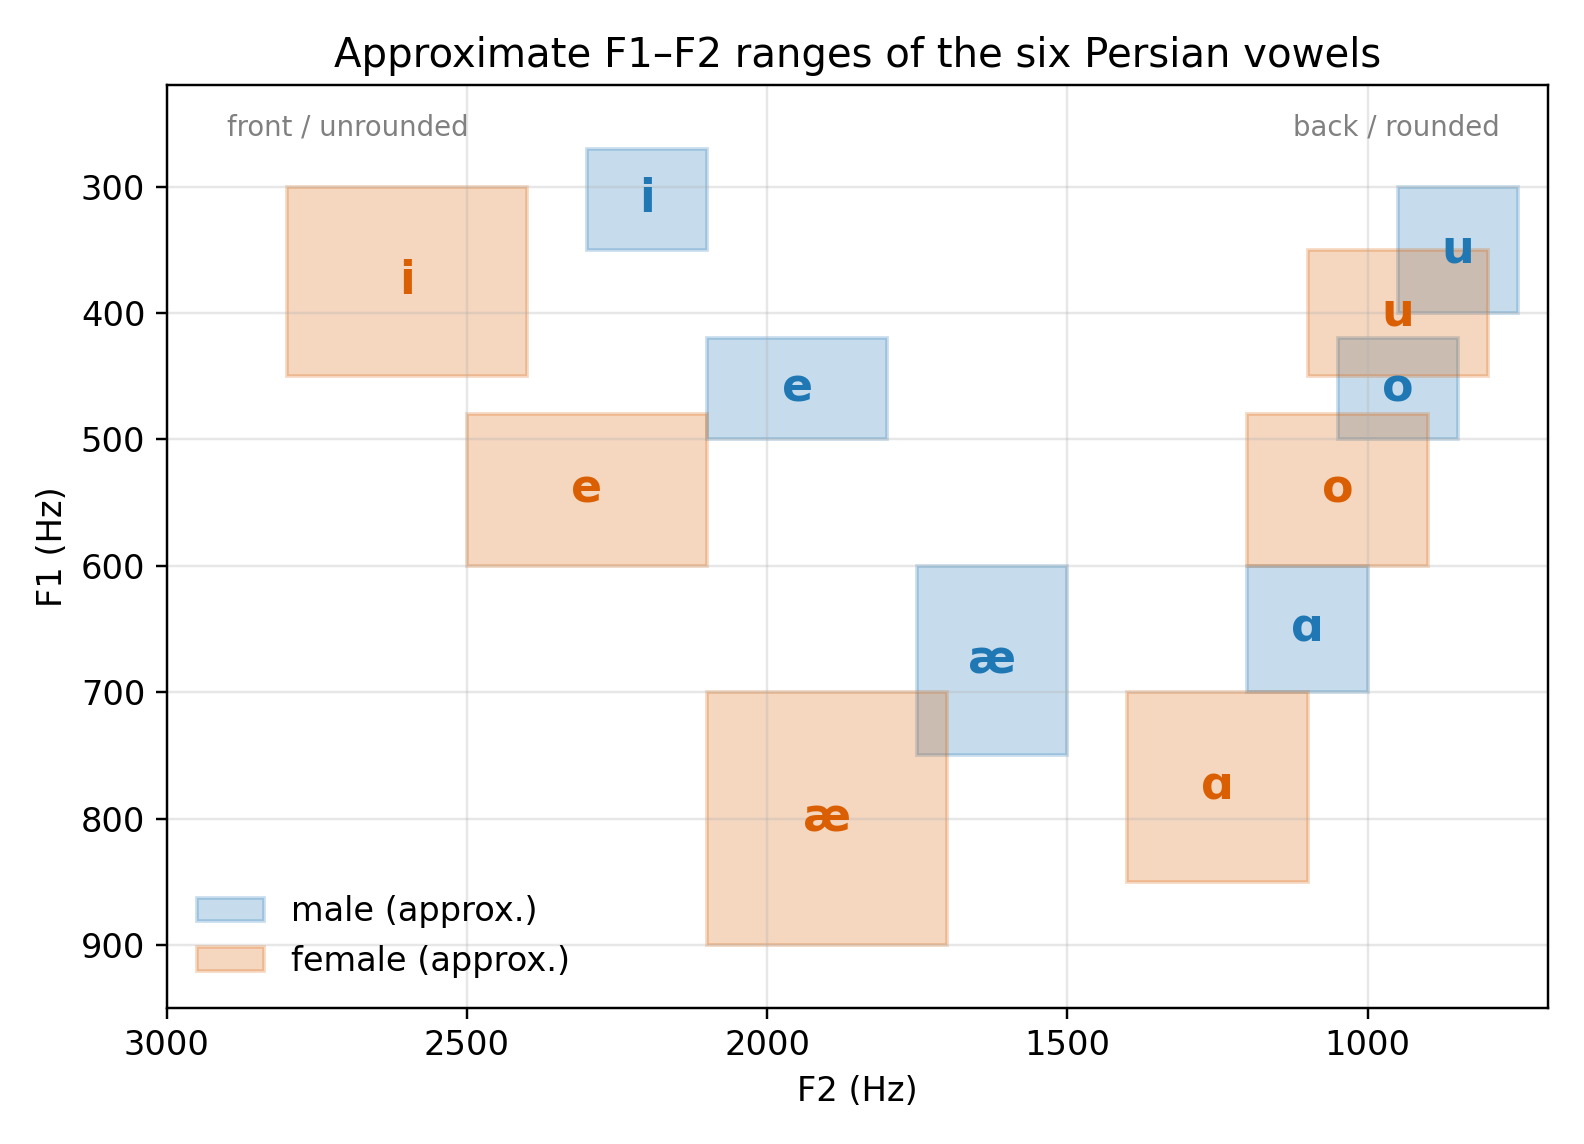
\includegraphics[width=0.75\textwidth]{../assets/figures/ch04-persian-vowel-chart.png}
  \caption{نمودار \eng{F1–F2} شش واکهٔ فارسی بر پایهٔ جدول بالا؛ مستطیل‌ها دامنهٔ مردان (آبی) و زنان (نارنجی) را نشان می‌دهند. محورها معکوس و مقادیر تقریبی‌اند (شکل افزوده).}
\end{figure}

\subsection{تفاوت فضای واکه‌ای در گروه‌های مختلف}
فضای واکه‌ای برای همه یکسان نیست و می‌توان آن را جداگانه برای کودکان و بزرگسالان، زنان و مردان، زبان‌های مختلف و افراد دارای اختلال گفتار استخراج کرد. انتظار داریم رابطهٔ کلی «\eng{F1} با ارتفاع و \eng{F2} با جلوآمدگی» حفظ شود، اما دامنهٔ عددی و پراکندگی تغییر کند. برای مقایسهٔ بین گویندگان معمولاً فرمنت‌ها نرمال می‌شوند، مثلاً با روش \eng{Lobanov}: $z=(F-\mu)/\sigma$ برای هر گوینده و هر فرمنت.

\subsection{مساحت فضای واکه‌ای (\eng{VSA})}
برای تبدیل «گستردگی فضای واکه‌ای» به یک عدد، مساحت چندضلعی واکه‌های گوشه در نمودار \eng{F1–F2} را حساب می‌کنیم (مقالهٔ \eng{Sandoval} و همکاران، ۲۰۱۳: چهار واکهٔ گوشه یا سه واکهٔ \eng{/a, i, u/} برای مثلث، با اندازه‌گیری در ۵۰ درصد مدت واکه و میانگین‌گیری). \eng{VSA} نمایندهٔ آکوستیکی جابه‌جایی اندام‌های گفتار است و در گفتار واضح‌تر بزرگ‌تر است.

\begin{definitionbox}{محاسبهٔ \eng{VSA} با فرمول شوله‌یس (\eng{Shoelace})}
اگر رأس‌های چندضلعی با ترتیب پیرامونی $(F_{2,k},F_{1,k})$ باشند:
\[
\text{\lr{VSA}}=\frac12\left|\sum_{k=1}^{n}\bigl(F_{2,k}\,F_{1,k+1}-F_{2,k+1}\,F_{1,k}\bigr)\right|\quad(\text{Hz}^2),\qquad k=n+1\equiv 1.
\]
برای مثلث \eng{(i, a, u)}:
\[
\text{\lr{VSA}}_{\triangle}=\frac12\left|F_{1,i}(F_{2,a}-F_{2,u})+F_{1,a}(F_{2,u}-F_{2,i})+F_{1,u}(F_{2,i}-F_{2,a})\right|.
\]
\end{definitionbox}

\begin{addedbox}{مثال عددی: \eng{VSA} مثلثی مردان فارسی‌زبان}
مرکز دامنه‌های جدول مردان: \eng{/i/} با $(F_1,F_2)=(310,\,2200)$، \eng{/ɑ/} با $(650,\,1100)$ و \eng{/u/} با $(350,\,850)$ هرتز.
\begin{align*}
\text{\lr{VSA}}_{\triangle}&=\tfrac12\bigl|310(1100-850)+650(850-2200)+350(2200-1100)\bigr|\\
&=\tfrac12\bigl|77\,500-877\,500+385\,000\bigr|=207\,500\ \text{Hz}^2.
\end{align*}
\textbf{اثر متمرکزشدن:} اگر هر فاصله از مرکز ثقل ۲۰ درصد کم شود (ضریب $0.8$)، چون مساحت با مربع ضریب مقیاس عوض می‌شود، مساحت جدید $0.8^2\times207\,500=132\,800\ \text{Hz}^2$ است، یعنی حدود ۳۶ درصد کاهش. پس \eng{VSA} به متمرکز شدن واکه‌ها حساس است. (شاخص نسبتی \eng{VAI} از \eng{Sapir} و همکاران ۲۰۱۰ برای کاهش وابستگی به اندازهٔ مجرا پیشنهاد شده و با متمرکزشدن کاهش می‌یابد.)
\end{addedbox}

\section{همخوان‌ها در اسپکتروگرام}
یکی از دانشجویان پرسید آیا این تحلیل فقط برای واکه‌هاست. پاسخ استاد: همخوان‌ها هم ویژگی‌های آکوستیکی خاص خود را دارند و در اسپکتروگرام قابل بررسی‌اند، اما تمرکز فعلی روی واکه‌هاست.

\begin{assignmentbox}{تمرین پیشنهادی استاد}
بررسی کنید همخوان‌ها چگونه در اسپکتروگرام دیده می‌شوند و آیا با آواشناسی تولیدی هماهنگ‌اند. روی تخته: اسپکتروگرام با \textbf{سکوت} (شیوهٔ تولید) و نحوهٔ \textbf{خم‌شدن و جهش فرمنت‌ها} و \textbf{مرکز فرکانسی نویز} (جایگاه تولید)، حرکات فیزیکی اندام‌های گفتاری را کدگذاری می‌کند. به‌خصوص این موارد را ببینید:
\begin{itemize}
  \item سکوت یا انسداد پیش از برخی همخوان‌ها؛
  \item انفجار (\eng{Burst}) در انسدادی‌هایی مانند \eng{/b/} و \eng{/p/};
  \item تغییر شکل فرمنت‌ها هنگام گذار از همخوان به واکه (\eng{Formant Transitions}).
\end{itemize}
\end{assignmentbox}

\section{کاربردهای فضای واکه‌ای}
استاد از دانشجویان پرسید فضای واکه‌ای چه کاربردی دارد. پاسخ‌های اولیه (تشخیص واکه، پیش‌پردازش) کافی نبود: فضای واکه‌ای قبل از هر چیز ابزار \emph{تحلیل ساختار تولید گفتار}، مقایسهٔ گروه‌ها و شناسایی الگوهای متفاوت است. سه کاربرد اصلی روی تخته بود.

\subsection{گفتاردرمانی و بازخورد زیستی تصویری}
در \term{بیوفیدبک تصویری}{Visual Biofeedback} برای کودکان دارای اختلال گفتار، ناشنوایان یا افراد مبتلا به سندرم داون، نمایشگری زنده نقطهٔ \eng{F1–F2} گفتار فرد را نشان می‌دهد و او می‌کوشد آن را با حرکت زبان به ناحیهٔ هدف برساند. مزیت: بازخورد از حالت صرفاً شنیداری به دیداری درمی‌آید. در گفتار کودکان و زنان ($f_0$ بالا) تخمین فرمنت ناپایدار است، پس بهتر است هدف را یک \emph{ناحیه} (بیضی دامنهٔ واکه) بگیریم، نه نقطه.

\subsection{تشخیص صدای جعلی (\eng{Deepfake})}
صدای سنتزشده می‌تواند برای گوش طبیعی باشد، اما این به معنای یکسان‌بودن همهٔ ویژگی‌های آکوستیکی و تولیدی با گفتار واقعی نیست. ایده: فرمنت‌های واکه‌ها را برای نمونهٔ واقعی و سنتزشده استخراج و فضای واکه‌ای (و هم‌بستگی الگوی تغییر \eng{F1} و \eng{F2}) را مقایسه کنیم. روی تخته: «تفاوت‌های بیومکانیکی در تلفظ مصوت‌ها بهترین ردپای مصنوعی‌بودن صدا هستند».

\begin{figure}[htbp]
  \centering
  \fbox{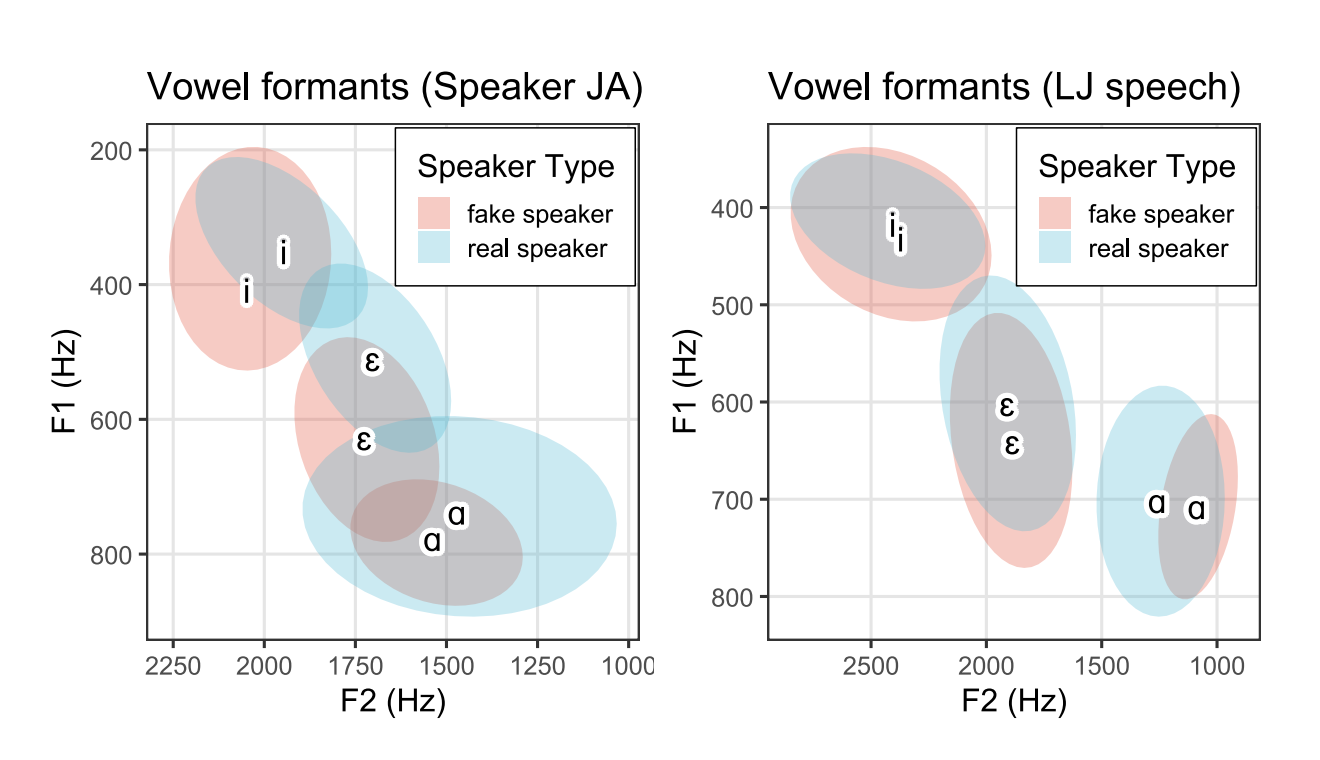
\includegraphics[width=0.55\textwidth]{../assets/figures/ch04-fake-real-vowels.png}}
  \caption{بیضی‌های \eng{F1–F2} چند واکه در صدای واقعی (آبی) و جعلی (قرمز) برای دو گوینده/پیکره، از مقالهٔ \eng{Conditional Speaker Normalization of Vocal Tract Shape Features for Robust Synthetic Speech Detection} (\eng{IEEE Access}، ۲۰۲۶) \textit{(برگرفته از تختهٔ کلاس)}}
\end{figure}

\begin{correctionbox}{«اثبات» جعل؟}
این روش‌ها شواهد آماری تولید می‌کنند، نه اثبات قطعی؛ در نمودار هم بسیاری از بیضی‌های واقعی و جعلی هم‌پوشانی زیادی دارند. استاد تأکید کرد گزارهٔ کلی «فرمنت‌ها فرق دارند» برای پژوهش کافی نیست؛ باید معلوم شود: (۱) دقیقاً کدام ویژگی تفاوت دارد، (۲) چگونه اندازه‌گیری می‌شود، (۳) آیا تکرارپذیر است، (۴) آیا تفکیک قابل‌اعتماد می‌دهد.
\end{correctionbox}

\textbf{مقاوم‌سازی مدل (\eng{Robustness}):} اگر نقاط ضعف مدل را بشناسیم (مثلاً ضعف در برخی واکه‌ها)، از همان داده‌ها بیشتر جمع می‌کنیم؛ روش‌های مرتبط: \eng{Data Augmentation}، \eng{Hard Example Mining} و \eng{Adversarial Training}. تحلیل فضای واکه‌ای می‌تواند یکی از راه‌های شناسایی این نقاط باشد.

\subsection{نشانگر زیستی دیجیتال (\eng{Digital Biomarker})}
\begin{definitionbox}{نشانگر زیستی دیجیتال}
ویژگی قابل‌اندازه‌گیری‌ای که با ابزارهای دیجیتال به دست می‌آید و دربارهٔ وضعیت یا تغییرات یک فرایند زیستی یا بالینی اطلاعات می‌دهد؛ مثلاً ویژگی‌های آکوستیکی گفتار برای دنبال‌کردن بیماری‌های عصبی مانند پارکینسون و دمانس.
\end{definitionbox}

در این بیماری‌ها \eng{F1} و \eng{F2} واکه‌ها به سمت مرکز فضای صوتی جمع می‌شوند (\term{متمرکزشدن}{Centralization}) و مساحت فضای واکه‌ای کوچک می‌شود. اندازه‌گیری مکرر در طول زمان می‌تواند تغییراتی را نشان دهد که شنوندهٔ عادی هنوز نمی‌شنود. روند پایش: ضبط دوره‌ای واکه‌ها یا جمله‌های ثابت $\leftarrow$ استخراج فرمنت $\leftarrow$ ساخت فضای واکه‌ای و اندازه‌گیری گستردگی $\leftarrow$ مقایسه با نمونه‌های قبلی همان فرد $\leftarrow$ در صورت تغییر قابل‌توجه، ارجاع به متخصص. استاد ایدهٔ سامانه‌ای مبتنی بر \textbf{تلفن همراه} برای این پایش را مطرح کرد. (مقالهٔ \eng{Sandoval} الگوریتمی برای تخمین خودکار \eng{VSA} از گفتار پیوسته ارائه می‌کند.)

\begin{figure}[htbp]
\centering
\begin{tikzpicture}[rtl, scale=1.0]
  \begin{scope}[xshift=6cm]
    \draw[fill=blue!15, draw=blue!60!black, thick] (0,0) -- (3,0.2) -- (2.3,2.5) -- cycle;
    \node[font=\small] at (1.8,-0.55) {فضای گسترده};
    \node[font=\small] at (1.8,-1.05) {تمایز بیشتر واکه‌ها};
    \node[font=\scriptsize] at (-0.2,-0.2) {\lr{/i/}};
    \node[font=\scriptsize] at (3.3,0.2) {\lr{/u/}};
    \node[font=\scriptsize] at (2.3,2.8) {\lr{/a/}};
  \end{scope}
  \begin{scope}
    \draw[fill=orange!20, draw=orange!70!black, thick] (0.8,0.65) -- (2.2,0.75) -- (1.9,1.7) -- cycle;
    \node[font=\small] at (1.5,-0.55) {فضای متمرکز};
    \node[font=\small] at (1.5,-1.05) {کاهش فاصلهٔ واکه‌ها};
    \node[font=\scriptsize] at (0.5,0.55) {\lr{/i/}};
    \node[font=\scriptsize] at (2.5,0.75) {\lr{/u/}};
    \node[font=\scriptsize] at (1.9,2.0) {\lr{/a/}};
  \end{scope}
  \draw[-{Stealth}, thick] (5.2,1.0) -- (3.9,1.0);
\end{tikzpicture}
\caption{نمایش شماتیک متمرکزشدن فضای واکه‌ای: مثلث واکه‌ها کوچک می‌شود و به مرکز نزدیک می‌شود (شکل افزوده).}
\end{figure}

\begin{correctionbox}{نشانگر زیستی دیجیتال ابزار تشخیص قطعی نیست}
شواهد پژوهشی کاهش \eng{VSA} یا \eng{VAI} را در برخی افراد مبتلا به پارکینسون و سایر دیزآرتری‌های حرکتی نشان می‌دهند، ولی اثر آن در همهٔ بیماران و مراحل یکسان نیست و برای دمانس شواهد ضعیف‌تر است. این شاخص‌ها به‌تنهایی تشخیص قطعی نیستند و به اعتبارسنجی بالینی و تفسیر متخصص نیاز دارند؛ سن، جنس، خستگی، کیفیت میکروفون و نویز نیز \eng{VSA} را تغییر می‌دهند.
\end{correctionbox}

\section{جمع‌بندی}
با اندازه‌گیری \eng{F1} و \eng{F2} در \eng{Praat} می‌توان بازنمایی‌ای از الگوی تولید واکه‌ها ساخت. با برچسب‌گذاری \eng{TextGrid} و بازهٔ هر واکه، جدول فرمنت‌ها برای هر گروه تهیه و در نمودار \eng{F1–F2} با محورهای معکوس فضای واکه‌ای شکل می‌گیرد. این بازنمایی امکان مقایسهٔ گروه‌ها، گفتاردرمانی تصویری، تشخیص صدای مصنوعی و پایش تغییرات گفتار را می‌دهد، اما همهٔ این کاربردها اعتبارسنجی دقیق و تفسیر محتاطانه می‌خواهند.

\begin{exambox}{نکات مهم برای مرور و امتحان}
\begin{center}
\small
\begin{tabular}{p{3.6cm}p{10cm}}
\toprule
مفهوم & نکتهٔ اصلی \\
\midrule
فرکانس پایه و \eng{Magnitude} & $f_0=1/T$، مربوط به منبع؛ \eng{Magnitude} اندازهٔ ضریب فوریه است، نه دامنهٔ زمانی \\
تعامد و هارمونیک‌ها & ضرب داخلی صفر؛ هارمونیک‌ها مضرب‌های صحیح $f_0$ (موج مربعی: فقط فرد) \\
فرمنت‌ها & نواحی تشدید مجرا (فیلتر)؛ تخمین با \eng{LPC} \\
\eng{Wideband} / \eng{Narrowband} & تفکیک زمانی (فرمنت) در برابر تفکیک فرکانسی (هارمونیک) \\
\eng{F1} و \eng{F2} & \eng{F1} معکوس با ارتفاع زبان؛ \eng{F2} مستقیم با جلو آمدن زبان و کاهش‌یافته با گردی لب \\
\eng{Praat} و \eng{TextGrid} & ضبط، تحلیل و استخراج فرمنت؛ لایه‌های \eng{Word}، \eng{Syllable}، \eng{Phoneme} \\
فضای واکه‌ای & نمودار \eng{F1–F2} با هر دو محور معکوس؛ برای هر گروه جداگانه \\
\eng{ASR} + بازبینی انسانی & ساخت سریع‌تر پیکره؛ مستندسازی برچسب‌گذاری ضروری \\
\eng{VSA} & مساحت چندضلعی واکه‌های گوشه؛ کوچک‌شدن = متمرکزشدن \\
کاربردها & گفتاردرمانی (بیوفیدبک تصویری)، تشخیص جعل، نشانگر زیستی دیجیتال \\
\bottomrule
\end{tabular}
\end{center}
\textbf{زنجیرهٔ جلسه:} سیگنال صوتی $\leftarrow$ ویژگی‌های آکوستیکی (\eng{Pitch}، طیف، فرمنت) $\leftarrow$ اندازه‌گیری \eng{F1}/\eng{F2} در \eng{Praat} $\leftarrow$ ساخت فضای واکه‌ای $\leftarrow$ مقایسه با مرجع یا گروه‌های دیگر $\leftarrow$ کاربردهای پژوهشی و عملی.
\end{exambox}
